\chapter{Implementation}
In this chapter it is described in details the framework that it has been implemented for assess the SQL-compliance for current DBMSs.

\section{Implementation}
This chapter describes the framework that is implemented for assessing the SQL-compliance of current DBMSs.

The framework is divided into three different tools as introduced in the previous chapter. The first two tools are implemented in the Java programming language and the third one is implemented in the Python programming language which is an open-source project that can generate random realistic data.  This project uses Java programming language since it is very popular and it can be used to build cross-platform systems. The complete framework consists of twenty java classes. 


 \begin{figure} 
      \centering
      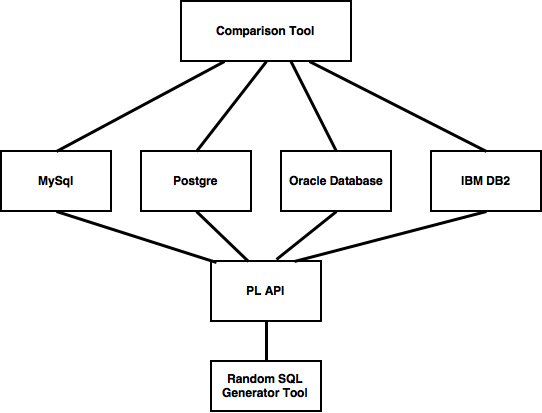
\includegraphics[width=\textwidth,height=6cm]{Images/1-implemen_detail}
      \caption{Random SQL Generator Architecture}
      \label{fig:counting-methods}
  \end{figure}

\subsection{Random SQL generator engine}
An important component of the framework is the random SQL query generator tool which is used to generate random SQL queries for assessing modern DBMSs. The SQL language consists of numerous SQL commands and therefore some of them are simple in terms of their usage such as ‘SELECT...FROM...WHERE’ where some others are more trickier such as ‘GROUP BY’, ‘HAVING’ or aggregation functions such as MAX, ‘COUNT’ or AVG. These SQL commands need to be properly generated and syntactically correct in order to avoid syntax or semantic errors.. As a result, for generating meaningful and syntactically valid queries, the current implementation of the generator tool must take into consideration table and attribute Naming, data type compatibility and projection.

In addition, the tool has been designed in a modular way for reusability and therefore new systems can easily extend it without the need of changing the whole structure of the tool.

Moreover, an important decision that is taken is with regards to the internal implementation of the generator tool, in order to make it feasible to generate more valid and syntactically correct SQL queries. Hence, an internal representation is implemented with each of its classes responsible for generating a different SQL clause that contributes to the overall query. For example, one of the java classes generates the SELECT clause. Having different classes for each SQL statement makes it easier to extend the tool in order to add new functionality and at the same time there is no need to change other parts of the tool. The final SQL query is converted to an SQL string which then is executed to the current DBMSs with the contribution of the comparison tool. An important note is that it is not feasible to generate SQL strings directly because the attribute names and data types need to be tracked first. If SQL strings were to be used, it would not be possible to check if a variable mentioned in the ‘WHERE’ clause is also mentioned in the ‘FROM’ clause or if that variable comes as a parameter from an external query. Thus, there is a need to track attributes for each clause and in order to achieve that, LinkedList and HashMap data-structures were used.


\subsection{Configuration file}
The generator tool also includes a configuration file for partially controlling the random SQL queries and a detailed explanation is given as follows: The configuration file is used to provide information to the generator tool. Therefore, many parameters can be specified from the configuration file. Below, the format of the configuration file and subsequently a comprehensive explanation is given  for every parameter. 


\begin{mdframed}[backgroundcolor=gray!20] 
  This configuration file will be used to give various parameter
  \\ to the SQLEngine

  Maximum number of tables in the FROM STATEMENT
\\maxTablesFrom =3

  Maximum number of attributes in the SELECT STATEMENT
\\maxAttrSel =5

  Maximun number of comparisons in the WHERE STATEMENT
\\maxCondWhere =7

 Represents the probability of having constants or NULL comparison \\ in the WHERE STATEMENT
\\probWhrConst = 0.8

 nestLevel = 4
\end{mdframed}

Another important decision that should be taken into account is the provision of relations and attributes to the tool. An initial approach was to use them as parameters in the configuration file. Although, this approach works acceptably, the resulting tool lacks portability, especially when a DBMS has a large number of tables and columns. Hence, It will be time-consuming to give these parameters via the configuration file. Thus, an efficient approach is to retrieve the whole schema from DBMSs automatically. As a result, the implemented tool has the capability to automatically retrieve the whole schema for any DBMS just by providing the credential for connecting to the database in the configuration file.    

\hfill\newline
All the parameters are described as follow:
\begin{description}
   \item[$\bullet$ relations and attributes] =  parameters are used to provide to the generator tool the tables and columns for generating SQL queries according to the database schema. The current architecture has the capability to automatically retrieve the whole database schema from any DBMS by just providing the credentials in the configuration file such as user, pass and dbName parameters. 

\item[$\bullet$ MaxTablesFrom] = parameter is used to set an upper bound of the number of tables that a ‘FROM’ clause can have. If the upper bound is greater than the total number of tables in the schema, then the upper bound is automatically set to the total number of tables. 

\item[$\bullet$ MaxAttrSel] =  parameter indicates an upper bound of projections in the ‘SELECT’ clause. In other words, it is the total number of attributes that can be selected in the ‘SELECT’ clause.
 
\item[$\bullet$ MaxCondWhere]= parameter represents the total number of comparison that the ‘WHERE’ clause can have. 
 
\item[$\bullet$ ProbWhrConst] = parameter represents the probability of having comparisons with constant or ‘Null’ in the ‘WHERE’ clause. Therefore, a number between 0 and 1 can be given for this parameter.  

\item[$\bullet$ RepAlias]= parameter indicates the probability of having repetition of alias in the ‘SELECT’ clause. 

\item[$\bullet$ NestLevel]= parameter represents the maximum level of nesting that a query can have. For generating such a query many considerations should be taken into account. For example, we should track attributes for outer queries, because inner query can access outer attributes or attributes from its ‘FROM’ clause. The opposite is not true, meaning that we cannot access attributes from an inner query. 

\item[$\bullet$ ArithCompSel] = parameter represents the probability of having arithmetic comparisons in the ‘SELECT’ clause. 

\item[$\bullet$ Dinstinct ] = parameter represents the probability of the ‘DISTINCT’ command appearing in the SQL statement. 

\item[$\bullet$ StringInSel] = parameter indicates the probability of projecting an attribute of type String or having String functions in the ‘SELECT’ clause. 

\item[$\bullet$ StringInWhere] = parameter represents the probability of having String comparison in ‘WHERE’ clause. 
 
\end{description} 

It can be seen from the configuration file that many parameters of the random query generator can be controlled but, on the other hand, it does not imply that the diversity of SQL queries that can be generated is restricted. For example, an upper bound of tables that appear in the FROM clause can be set. In that way, having an enormous table size from cartesian product can be avoided.

In addition, it is not so common to have constant comparisons in an SQL query even though SQL Standard supports it. Thus, SQL queries which have constant comparisons are generated but only with a limited number based on the probability which is given in the configuration file.


\textbf{SQL Query generated by the random query generator} 

\begin{mdframed}[backgroundcolor=gray!20] 
SELECT r41.A AS A0
\\FROM r4 AS r41
\\WHERE 1 > 2
\end{mdframed}

\section{Comparison Tool} 
The generated SQL queries are evaluated on five different DBMSs as they were mentioned in the methodology chapter. The comparison tool (CT) takes into consideration all methods of accessing different databases so that the process of executing and comparing identical queries among all databases can be automated.

The CT is illustrated below and  a detailed explanation of its internal implementation is provided.
 \begin{figure} 
      \centering
      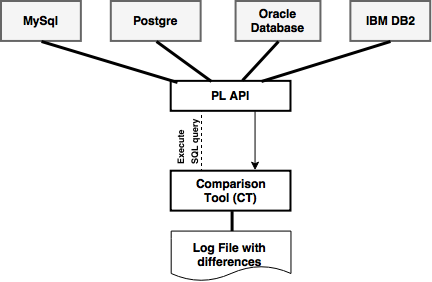
\includegraphics[width=\textwidth,height=6cm]{Images/2-ComparisonTool}
      \caption{Simple Architecture of Comparison Tool}
      \label{fig:counting-methods}
  \end{figure}

The tool is implemented in Java programming language and is one of the main components of the complete framework. Specifically, the CT is used to compare the results of each randomly generated query. As each DBMS uses various algorithms to evaluate each query, sometimes the results are identical but the order or format differs. As a consequence, for efficient comparison of the query results between DBMSs, the following approach is used: Initially, the query results are stored in a LinkedList, so that an efficient in-memory sorting algorithm can be performed, called Quicksort. In that way, the results among the DBMSs should be the same and a row by row comparison is performed to verify that they are identical. If a difference is found or a query raises an error, on one of the tested DBMSs, then a detailed explanation of the difference or the error message is recorded in the log file.


An important consideration for implementing this tool is its ease of reuse and extensibility by other systems or software. As each system needs its own credentials such as username, password and database name, a configuration file is created for providing these information to the CT. By doing so, the CT becomes portable and adaptable and a new system can be easily added. As shown in the experiments chapter, our approach can detect many important differences and issues. 

 \begin{figure} 
      \centering
      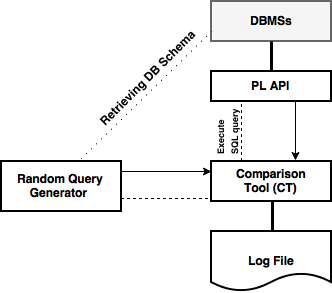
\includegraphics[width=\textwidth,height=6cm]{Images/3-ComparisonTool}
      \caption{Architecture of Comparison Tool}
      \label{fig:counting-methods}
  \end{figure}

\section{Random generated data}

Datafiller is a well-known open-source project that provides the capability of generating random data [3]. For our project, Datafiller will be used for generating a diversity of  database instances in order to evaluate all major DBMSs. More precisely, the Datafiller script generates random data, based on a an SQL  schema which is provided as a parameter and it takes into account constraints of that schema for generating valid data. For example, it takes into account the domain of each field and if each field should be unique, foreign key or primary key. Another important parameter is the df: null=rate\% which indicates the nullable rates. It necessary to test the behaviour of current DBMS in databases with nulls in order to evaluate whether all DBMSs behave in a similar fashion regarding null values.     

Additionally, more complex parameters can be provided as well, such as the number of tuples per table using --size SIZE parameter. It is worth mentioning that these parameters should be defined within the schema script and should start with ‘-- df’.  Furthermore, we can generate more realistic data by providing some information in the schema SQL script. For instance, if there is a field which represents a date, then we can provide a range in order for the Datafiller to generate dates only within that range. This can be achieved by specifying the following parameter: range -- df: start=year-month-day end=year-month-day next to the Date field. Subsequently, we need to add the --filter parameter while running the script. These are only some of the important parameters that the Datafiller provides but apart from these, it provides more sophisticated properties which are out of importance for our project.



 \begin{figure} 
      \centering
      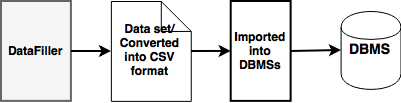
\includegraphics[width=\textwidth,height=2cm]{Images/4-Datafiller}
      \caption{Method of importing csv files}
      \label{fig:counting-methods}
  \end{figure}  


Datafiller supports data importing only into PostgreSQL and therefore, for our project we need to import the random generated data into five DBMSs. For this reason, we transform the data into CSV format, as all of them support importing data from CSV files.  

